% TODO: note about the notation being slightly different from that of the paper
\begin{figure}[ht]
	\centering
	\begin{subfigure}{.5\textwidth}
		\centering

		\begin{align*}
			\vh^\parent_i &= g^\parent{\left( \vh^\parent_{\parent(i)}, 
			\vx^{}_{\parent(i)} \right)}
			\\
					\vh^\leftsib_i &= g^\leftsib{\left( \vh^\leftsib_{\leftsib(i)}, 
					\vx^{}_{\leftsib(i)} \right)}
			\\
					\hpred_i &= \tanh{\left(\rmU^\parent \vh^\parent_i + \rmU^\leftsib 
					\vh^\leftsib\right)}
			\\
						p^\parent_i &= \sigma{\left(\rvu^\parent \cdot \hpred \right)}
			\\
						p^\leftsib_i &= \sigma{\left(\rvu^\leftsib \cdot \hpred \right)}
			\\
						\vo_i &= \softmax{\left(\rmW\hpred_i + \alpha_i\rvv^\parent + 
						\varphi_i\rvv^\leftsib \right)}
			\\
		\end{align*}

		\caption{A subfigure}\label{fig:broken_1}
	\end{subfigure}%
	\begin{subfigure}{.5\textwidth}
		\centering

		\tikzset{every picture/.style={line width=0.75pt}} %set default line width to 0.75pt

		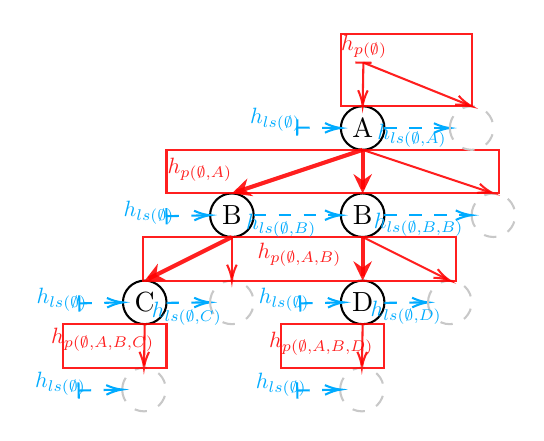
\begin{tikzpicture}[scale=0.7,x=0.75pt,y=0.75pt,yscale=-1,xscale=1]
		%uncomment if require: \path (0,336.6875); %set diagram left start at 0, and has height of 336.6875

		%Shape: Circle [id:dp5747539528933221] 
		\draw   (240,75) .. controls (240,66.72) and (246.72,60) .. (255,60) .. controls (263.28,60) and (270,66.72) .. (270,75) .. controls (270,83.28) and (263.28,90) .. (255,90) .. controls (246.72,90) and (240,83.28) .. (240,75) -- cycle ;
		%Shape: Circle [id:dp6584741963271383] 
		\draw   (150,135) .. controls (150,126.72) and (156.72,120) .. (165,120) .. controls (173.28,120) and (180,126.72) .. (180,135) .. controls (180,143.28) and (173.28,150) .. (165,150) .. controls (156.72,150) and (150,143.28) .. (150,135) -- cycle ;
		%Shape: Circle [id:dp42608384351679063] 
		\draw   (240,135) .. controls (240,126.72) and (246.72,120) .. (255,120) .. controls (263.28,120) and (270,126.72) .. (270,135) .. controls (270,143.28) and (263.28,150) .. (255,150) .. controls (246.72,150) and (240,143.28) .. (240,135) -- cycle ;
		%Shape: Circle [id:dp4039562507165959] 
		\draw   (90,195) .. controls (90,186.72) and (96.72,180) .. (105,180) .. controls (113.28,180) and (120,186.72) .. (120,195) .. controls (120,203.28) and (113.28,210) .. (105,210) .. controls (96.72,210) and (90,203.28) .. (90,195) -- cycle ;
		%Shape: Circle [id:dp6061665496522999] 
		\draw   (240,195) .. controls (240,186.72) and (246.72,180) .. (255,180) .. controls (263.28,180) and (270,186.72) .. (270,195) .. controls (270,203.28) and (263.28,210) .. (255,210) .. controls (246.72,210) and (240,203.28) .. (240,195) -- cycle ;
		%Straight Lines [id:da5328040663765743] 
		\draw [color={rgb, 255:red, 255; green, 0; blue, 0 }  ,draw opacity=0.88 ][line width=1.5]    (255,90) -- (167.85,119.05) ;
		\draw [shift={(165,120)}, rotate = 341.57] [fill={rgb, 255:red, 255; green, 0; blue, 0 }  ,fill opacity=0.88 ][line width=1.5]  [draw opacity=0] (13.4,-6.43) -- (0,0) -- (13.4,6.44) -- (8.9,0) -- cycle    ;

		%Straight Lines [id:da567244828908992] 
		\draw [color={rgb, 255:red, 255; green, 0; blue, 0 }  ,draw opacity=0.88 ][line width=1.5]    (255,90) -- (255,117) ;
		\draw [shift={(255,120)}, rotate = 270] [fill={rgb, 255:red, 255; green, 0; blue, 0 }  ,fill opacity=0.88 ][line width=1.5]  [draw opacity=0] (13.4,-6.43) -- (0,0) -- (13.4,6.44) -- (8.9,0) -- cycle    ;

		%Straight Lines [id:da20403721062923252] 
		\draw [color={rgb, 255:red, 255; green, 0; blue, 0 }  ,draw opacity=0.88 ][line width=1.5]    (165,150) -- (107.68,178.66) ;
		\draw [shift={(105,180)}, rotate = 333.43] [fill={rgb, 255:red, 255; green, 0; blue, 0 }  ,fill opacity=0.88 ][line width=1.5]  [draw opacity=0] (13.4,-6.43) -- (0,0) -- (13.4,6.44) -- (8.9,0) -- cycle    ;

		%Straight Lines [id:da25420509470673447] 
		\draw [color={rgb, 255:red, 255; green, 0; blue, 0 }  ,draw opacity=0.88 ][line width=1.5]    (255,150) -- (255,177) ;
		\draw [shift={(255,180)}, rotate = 270] [fill={rgb, 255:red, 255; green, 0; blue, 0 }  ,fill opacity=0.88 ][line width=1.5]  [draw opacity=0] (13.4,-6.43) -- (0,0) -- (13.4,6.44) -- (8.9,0) -- cycle    ;

		%Straight Lines [id:da060062721758333826] 
		\draw [color={rgb, 255:red, 255; green, 0; blue, 0 }  ,draw opacity=0.88 ]   (105,210) -- (104.53,238) ;
		\draw [shift={(104.5,240)}, rotate = 270.95] [color={rgb, 255:red, 255; green, 0; blue, 0 }  ,draw opacity=0.88 ][line width=0.75]    (10.93,-3.29) .. controls (6.95,-1.4) and (3.31,-0.3) .. (0,0) .. controls (3.31,0.3) and (6.95,1.4) .. (10.93,3.29)   ;

		%Straight Lines [id:da9112525130551028] 
		\draw [color={rgb, 255:red, 255; green, 0; blue, 0 }  ,draw opacity=0.88 ]   (255,210) -- (254.53,238) ;
		\draw [shift={(254.5,240)}, rotate = 270.95] [color={rgb, 255:red, 255; green, 0; blue, 0 }  ,draw opacity=0.88 ][line width=0.75]    (10.93,-3.29) .. controls (6.95,-1.4) and (3.31,-0.3) .. (0,0) .. controls (3.31,0.3) and (6.95,1.4) .. (10.93,3.29)   ;

		%Straight Lines [id:da42382449393367416] 
		\draw [color={rgb, 255:red, 255; green, 0; blue, 0 }  ,draw opacity=0.88 ]   (255,90) -- (343.1,119.37) ;
		\draw [shift={(345,120)}, rotate = 198.43] [color={rgb, 255:red, 255; green, 0; blue, 0 }  ,draw opacity=0.88 ][line width=0.75]    (10.93,-3.29) .. controls (6.95,-1.4) and (3.31,-0.3) .. (0,0) .. controls (3.31,0.3) and (6.95,1.4) .. (10.93,3.29)   ;

		%Shape: Circle [id:dp9771338101075551] 
		\draw  [color={rgb, 255:red, 200; green, 200; blue, 200 }  ,draw opacity=1 ][dash pattern={on 4.5pt off 4.5pt}] (330,135) .. controls (330,126.72) and (336.72,120) .. (345,120) .. controls (353.28,120) and (360,126.72) .. (360,135) .. controls (360,143.28) and (353.28,150) .. (345,150) .. controls (336.72,150) and (330,143.28) .. (330,135) -- cycle ;
		%Straight Lines [id:da75928763497055] 
		\draw [color={rgb, 255:red, 0; green, 171; blue, 255 }  ,draw opacity=1 ] [dash pattern={on 4.5pt off 4.5pt}]  (180,135) -- (238,135) ;
		\draw [shift={(240,135)}, rotate = 180] [color={rgb, 255:red, 0; green, 171; blue, 255 }  ,draw opacity=1 ][line width=0.75]    (10.93,-3.29) .. controls (6.95,-1.4) and (3.31,-0.3) .. (0,0) .. controls (3.31,0.3) and (6.95,1.4) .. (10.93,3.29)   ;

		%Straight Lines [id:da8384243170280115] 
		\draw [color={rgb, 255:red, 0; green, 171; blue, 255 }  ,draw opacity=1 ] [dash pattern={on 4.5pt off 4.5pt}]  (120,195.31) -- (148,195.02) ;
		\draw [shift={(150,195)}, rotate = 539.4] [color={rgb, 255:red, 0; green, 171; blue, 255 }  ,draw opacity=1 ][line width=0.75]    (10.93,-3.29) .. controls (6.95,-1.4) and (3.31,-0.3) .. (0,0) .. controls (3.31,0.3) and (6.95,1.4) .. (10.93,3.29)   ;

		%Shape: Circle [id:dp852651930656483] 
		\draw  [color={rgb, 255:red, 200; green, 200; blue, 200 }  ,draw opacity=1 ][dash pattern={on 4.5pt off 4.5pt}] (150,195) .. controls (150,186.72) and (156.72,180) .. (165,180) .. controls (173.28,180) and (180,186.72) .. (180,195) .. controls (180,203.28) and (173.28,210) .. (165,210) .. controls (156.72,210) and (150,203.28) .. (150,195) -- cycle ;
		%Straight Lines [id:da33797387516994126] 
		\draw [color={rgb, 255:red, 255; green, 0; blue, 0 }  ,draw opacity=0.88 ]   (165,150) -- (165,178) ;
		\draw [shift={(165,180)}, rotate = 270] [color={rgb, 255:red, 255; green, 0; blue, 0 }  ,draw opacity=0.88 ][line width=0.75]    (10.93,-3.29) .. controls (6.95,-1.4) and (3.31,-0.3) .. (0,0) .. controls (3.31,0.3) and (6.95,1.4) .. (10.93,3.29)   ;

		%Shape: Circle [id:dp7781216259767076] 
		\draw  [color={rgb, 255:red, 200; green, 200; blue, 200 }  ,draw opacity=1 ][dash pattern={on 4.5pt off 4.5pt}] (89.5,255) .. controls (89.5,246.72) and (96.22,240) .. (104.5,240) .. controls (112.78,240) and (119.5,246.72) .. (119.5,255) .. controls (119.5,263.28) and (112.78,270) .. (104.5,270) .. controls (96.22,270) and (89.5,263.28) .. (89.5,255) -- cycle ;
		%Straight Lines [id:da7533173940295115] 
		\draw [color={rgb, 255:red, 0; green, 171; blue, 255 }  ,draw opacity=1 ] [dash pattern={on 4.5pt off 4.5pt}]  (270,195.31) -- (298,195.02) ;
		\draw [shift={(300,195)}, rotate = 539.4] [color={rgb, 255:red, 0; green, 171; blue, 255 }  ,draw opacity=1 ][line width=0.75]    (10.93,-3.29) .. controls (6.95,-1.4) and (3.31,-0.3) .. (0,0) .. controls (3.31,0.3) and (6.95,1.4) .. (10.93,3.29)   ;

		%Shape: Circle [id:dp739418235900434] 
		\draw  [color={rgb, 255:red, 200; green, 200; blue, 200 }  ,draw opacity=1 ][dash pattern={on 4.5pt off 4.5pt}] (300,195) .. controls (300,186.72) and (306.72,180) .. (315,180) .. controls (323.28,180) and (330,186.72) .. (330,195) .. controls (330,203.28) and (323.28,210) .. (315,210) .. controls (306.72,210) and (300,203.28) .. (300,195) -- cycle ;
		%Straight Lines [id:da5061830263709963] 
		\draw [color={rgb, 255:red, 255; green, 0; blue, 0 }  ,draw opacity=0.88 ]   (255,150) -- (313.21,179.11) ;
		\draw [shift={(315,180)}, rotate = 206.57] [color={rgb, 255:red, 255; green, 0; blue, 0 }  ,draw opacity=0.88 ][line width=0.75]    (10.93,-3.29) .. controls (6.95,-1.4) and (3.31,-0.3) .. (0,0) .. controls (3.31,0.3) and (6.95,1.4) .. (10.93,3.29)   ;

		%Shape: Circle [id:dp4830940102467898] 
		\draw  [color={rgb, 255:red, 200; green, 200; blue, 200 }  ,draw opacity=1 ][dash pattern={on 4.5pt off 4.5pt}] (239.5,255) .. controls (239.5,246.72) and (246.22,240) .. (254.5,240) .. controls (262.78,240) and (269.5,246.72) .. (269.5,255) .. controls (269.5,263.28) and (262.78,270) .. (254.5,270) .. controls (246.22,270) and (239.5,263.28) .. (239.5,255) -- cycle ;
		%Straight Lines [id:da8687951733883794] 
		\draw [color={rgb, 255:red, 255; green, 0; blue, 0 }  ,draw opacity=0.88 ]   (255.5,30) -- (255.03,58) ;
		\draw [shift={(255,60)}, rotate = 270.95] [color={rgb, 255:red, 255; green, 0; blue, 0 }  ,draw opacity=0.88 ][line width=0.75]    (10.93,-3.29) .. controls (6.95,-1.4) and (3.31,-0.3) .. (0,0) .. controls (3.31,0.3) and (6.95,1.4) .. (10.93,3.29)   ;
		\draw [shift={(255.5,30)}, rotate = 270.95] [color={rgb, 255:red, 255; green, 0; blue, 0 }  ,draw opacity=0.88 ][line width=0.75]    (0,5.59) -- (0,-5.59)   ;
		%Straight Lines [id:da2320681357192822] 
		\draw [color={rgb, 255:red, 0; green, 171; blue, 255 }  ,draw opacity=1 ] [dash pattern={on 4.5pt off 4.5pt}]  (210,74.69) -- (238,74.98) ;
		\draw [shift={(240,75)}, rotate = 180.6] [color={rgb, 255:red, 0; green, 171; blue, 255 }  ,draw opacity=1 ][line width=0.75]    (10.93,-3.29) .. controls (6.95,-1.4) and (3.31,-0.3) .. (0,0) .. controls (3.31,0.3) and (6.95,1.4) .. (10.93,3.29)   ;
		\draw [shift={(210,74.69)}, rotate = 180.6] [color={rgb, 255:red, 0; green, 171; blue, 255 }  ,draw opacity=1 ][line width=0.75]    (0,5.59) -- (0,-5.59)   ;
		%Straight Lines [id:da9763574735032972] 
		\draw [color={rgb, 255:red, 0; green, 171; blue, 255 }  ,draw opacity=1 ] [dash pattern={on 4.5pt off 4.5pt}]  (60,195.69) -- (88,195.05) ;
		\draw [shift={(90,195)}, rotate = 538.69] [color={rgb, 255:red, 0; green, 171; blue, 255 }  ,draw opacity=1 ][line width=0.75]    (10.93,-3.29) .. controls (6.95,-1.4) and (3.31,-0.3) .. (0,0) .. controls (3.31,0.3) and (6.95,1.4) .. (10.93,3.29)   ;
		\draw [shift={(60,195.69)}, rotate = 538.69] [color={rgb, 255:red, 0; green, 171; blue, 255 }  ,draw opacity=1 ][line width=0.75]    (0,5.59) -- (0,-5.59)   ;
		%Straight Lines [id:da46410867028671343] 
		\draw [color={rgb, 255:red, 0; green, 171; blue, 255 }  ,draw opacity=1 ] [dash pattern={on 4.5pt off 4.5pt}]  (120,135.69) -- (148,135.05) ;
		\draw [shift={(150,135)}, rotate = 538.69] [color={rgb, 255:red, 0; green, 171; blue, 255 }  ,draw opacity=1 ][line width=0.75]    (10.93,-3.29) .. controls (6.95,-1.4) and (3.31,-0.3) .. (0,0) .. controls (3.31,0.3) and (6.95,1.4) .. (10.93,3.29)   ;
		\draw [shift={(120,135.69)}, rotate = 538.69] [color={rgb, 255:red, 0; green, 171; blue, 255 }  ,draw opacity=1 ][line width=0.75]    (0,5.59) -- (0,-5.59)   ;
		%Shape: Rectangle [id:dp9442762725540359] 
		\draw  [color={rgb, 255:red, 255; green, 0; blue, 0 }  ,draw opacity=0.88 ] (120,90) -- (349,90) -- (349,120) -- (120,120) -- cycle ;
		%Shape: Rectangle [id:dp46916019889141514] 
		\draw  [color={rgb, 255:red, 255; green, 0; blue, 0 }  ,draw opacity=0.88 ] (104,150) -- (319,150) -- (319,180) -- (104,180) -- cycle ;
		%Straight Lines [id:da250704382329064] 
		\draw [color={rgb, 255:red, 0; green, 171; blue, 255 }  ,draw opacity=1 ] [dash pattern={on 4.5pt off 4.5pt}]  (59.5,255.69) -- (87.5,255.05) ;
		\draw [shift={(89.5,255)}, rotate = 538.69] [color={rgb, 255:red, 0; green, 171; blue, 255 }  ,draw opacity=1 ][line width=0.75]    (10.93,-3.29) .. controls (6.95,-1.4) and (3.31,-0.3) .. (0,0) .. controls (3.31,0.3) and (6.95,1.4) .. (10.93,3.29)   ;
		\draw [shift={(59.5,255.69)}, rotate = 538.69] [color={rgb, 255:red, 0; green, 171; blue, 255 }  ,draw opacity=1 ][line width=0.75]    (0,5.59) -- (0,-5.59)   ;
		%Straight Lines [id:da7469552192135425] 
		\draw [color={rgb, 255:red, 0; green, 171; blue, 255 }  ,draw opacity=1 ] [dash pattern={on 4.5pt off 4.5pt}]  (210,255.69) -- (238,255.05) ;
		\draw [shift={(240,255)}, rotate = 538.69] [color={rgb, 255:red, 0; green, 171; blue, 255 }  ,draw opacity=1 ][line width=0.75]    (10.93,-3.29) .. controls (6.95,-1.4) and (3.31,-0.3) .. (0,0) .. controls (3.31,0.3) and (6.95,1.4) .. (10.93,3.29)   ;
		\draw [shift={(210,255.69)}, rotate = 538.69] [color={rgb, 255:red, 0; green, 171; blue, 255 }  ,draw opacity=1 ][line width=0.75]    (0,5.59) -- (0,-5.59)   ;
		%Straight Lines [id:da577886155294407] 
		\draw [color={rgb, 255:red, 0; green, 171; blue, 255 }  ,draw opacity=1 ] [dash pattern={on 4.5pt off 4.5pt}]  (212,195.69) -- (240,195.05) ;
		\draw [shift={(242,195)}, rotate = 538.69] [color={rgb, 255:red, 0; green, 171; blue, 255 }  ,draw opacity=1 ][line width=0.75]    (10.93,-3.29) .. controls (6.95,-1.4) and (3.31,-0.3) .. (0,0) .. controls (3.31,0.3) and (6.95,1.4) .. (10.93,3.29)   ;
		\draw [shift={(212,195.69)}, rotate = 538.69] [color={rgb, 255:red, 0; green, 171; blue, 255 }  ,draw opacity=1 ][line width=0.75]    (0,5.59) -- (0,-5.59)   ;
		%Straight Lines [id:da7835054268870489] 
		\draw [color={rgb, 255:red, 0; green, 171; blue, 255 }  ,draw opacity=1 ] [dash pattern={on 4.5pt off 4.5pt}]  (270,135) -- (328,135) ;
		\draw [shift={(330,135)}, rotate = 180] [color={rgb, 255:red, 0; green, 171; blue, 255 }  ,draw opacity=1 ][line width=0.75]    (10.93,-3.29) .. controls (6.95,-1.4) and (3.31,-0.3) .. (0,0) .. controls (3.31,0.3) and (6.95,1.4) .. (10.93,3.29)   ;

		%Straight Lines [id:da8246021494117906] 
		\draw [color={rgb, 255:red, 0; green, 171; blue, 255 }  ,draw opacity=1 ] [dash pattern={on 4.5pt off 4.5pt}]  (270,75) -- (313,75) ;
		\draw [shift={(315,75)}, rotate = 180] [color={rgb, 255:red, 0; green, 171; blue, 255 }  ,draw opacity=1 ][line width=0.75]    (10.93,-3.29) .. controls (6.95,-1.4) and (3.31,-0.3) .. (0,0) .. controls (3.31,0.3) and (6.95,1.4) .. (10.93,3.29)   ;

		%Shape: Circle [id:dp14086195915841282] 
		\draw  [color={rgb, 255:red, 200; green, 200; blue, 200 }  ,draw opacity=1 ][dash pattern={on 4.5pt off 4.5pt}] (315,75) .. controls (315,66.72) and (321.72,60) .. (330,60) .. controls (338.28,60) and (345,66.72) .. (345,75) .. controls (345,83.28) and (338.28,90) .. (330,90) .. controls (321.72,90) and (315,83.28) .. (315,75) -- cycle ;
		%Straight Lines [id:da5272161259387991] 
		\draw [color={rgb, 255:red, 255; green, 0; blue, 0 }  ,draw opacity=0.88 ]   (255.5,30) -- (328.14,59.25) ;
		\draw [shift={(330,60)}, rotate = 201.93] [color={rgb, 255:red, 255; green, 0; blue, 0 }  ,draw opacity=0.88 ][line width=0.75]    (10.93,-3.29) .. controls (6.95,-1.4) and (3.31,-0.3) .. (0,0) .. controls (3.31,0.3) and (6.95,1.4) .. (10.93,3.29)   ;

		%Shape: Rectangle [id:dp7842787512852565] 
		\draw  [color={rgb, 255:red, 255; green, 0; blue, 0 }  ,draw opacity=0.88 ] (240,10.31) -- (330,10.31) -- (330,60) -- (240,60) -- cycle ;
		%Shape: Rectangle [id:dp6269636709503503] 
		\draw  [color={rgb, 255:red, 255; green, 0; blue, 0 }  ,draw opacity=0.88 ] (49,210) -- (120,210) -- (120,240) -- (49,240) -- cycle ;
		%Shape: Rectangle [id:dp035044351208313174] 
		\draw  [color={rgb, 255:red, 255; green, 0; blue, 0 }  ,draw opacity=0.88 ] (199,210) -- (270,210) -- (270,240) -- (199,240) -- cycle ;

		% Text Node
		\draw (255,75) node  [align=left] {A};
		% Text Node
		\draw (165,135) node  [align=left] {B};
		% Text Node
		\draw (255,195) node  [align=left] {D};
		% Text Node
		\draw (105,195) node  [align=left] {C};
		% Text Node
		\draw (255,135) node  [align=left] {B};
		% Text Node
		\draw (195,69.5) node [scale=0.8,color={rgb, 255:red, 0; green, 171; blue, 255 }  ,opacity=1 ] [align=left] {$\displaystyle h_{ls( \emptyset )}$};
		% Text Node
		\draw (47,251) node [scale=0.8,color={rgb, 255:red, 0; green, 171; blue, 255 }  ,opacity=1 ] [align=left] {$\displaystyle h_{ls( \emptyset )}$};
		% Text Node
		\draw (143,103.5) node [scale=0.8,color={rgb, 255:red, 255; green, 0; blue, 0 }  ,opacity=0.88 ] [align=left] {$\displaystyle h_{p( \emptyset ,A)}$};
		% Text Node
		\draw (256,19) node [scale=0.8,color={rgb, 255:red, 255; green, 0; blue, 0 }  ,opacity=0.88 ] [align=left] {$\displaystyle h_{p( \emptyset )}$};
		% Text Node
		\draw (211.5,162) node [scale=0.8,color={rgb, 255:red, 255; green, 0; blue, 0 }  ,opacity=0.88 ] [align=left] {$\displaystyle h_{p( \emptyset ,A,B)}$};
		% Text Node
		\draw (76,221) node [scale=0.8,color={rgb, 255:red, 255; green, 0; blue, 0 }  ,opacity=0.88 ] [align=left] {$\displaystyle h_{p( \emptyset ,A,B,C)}$};
		% Text Node
		\draw (48,193.5) node [scale=0.8,color={rgb, 255:red, 0; green, 171; blue, 255 }  ,opacity=1 ] [align=left] {$\displaystyle h_{ls( \emptyset )}$};
		% Text Node
		\draw (108,133) node [scale=0.8,color={rgb, 255:red, 0; green, 171; blue, 255 }  ,opacity=1 ] [align=left] {$\displaystyle h_{ls( \emptyset )}$};
		% Text Node
		\draw (134,203) node [scale=0.8,color={rgb, 255:red, 0; green, 171; blue, 255 }  ,opacity=1 ] [align=left] {$\displaystyle h_{ls( \emptyset ,C)}$};
		% Text Node
		\draw (226.5,223.5) node [scale=0.8,color={rgb, 255:red, 255; green, 0; blue, 0 }  ,opacity=0.88 ] [align=left] {$\displaystyle h_{p( \emptyset ,A,B,D)}$};
		% Text Node
		\draw (199,252) node [scale=0.8,color={rgb, 255:red, 0; green, 171; blue, 255 }  ,opacity=1 ] [align=left] {$\displaystyle h_{ls( \emptyset )}$};
		% Text Node
		\draw (201,193) node [scale=0.8,color={rgb, 255:red, 0; green, 171; blue, 255 }  ,opacity=1 ] [align=left] {$\displaystyle h_{ls( \emptyset )}$};
		% Text Node
		\draw (285,202) node [scale=0.8,color={rgb, 255:red, 0; green, 171; blue, 255 }  ,opacity=1 ] [align=left] {$\displaystyle h_{ls( \emptyset ,D)}$};
		% Text Node
		\draw (293.5,141.5) node [scale=0.8,color={rgb, 255:red, 0; green, 171; blue, 255 }  ,opacity=1 ] [align=left] {$\displaystyle h_{ls( \emptyset ,B,B)}$};
		% Text Node
		\draw (120,138) node  [align=left] {$ $};
		% Text Node
		\draw (199,142) node [scale=0.8,color={rgb, 255:red, 0; green, 171; blue, 255 }  ,opacity=1 ] [align=left] {$\displaystyle h_{ls( \emptyset ,B)}$};
		% Text Node
		\draw (289,80.5) node [scale=0.8,color={rgb, 255:red, 0; green, 171; blue, 255 }  ,opacity=1 ] [align=left] {$\displaystyle h_{ls( \emptyset ,A)}$};


		\end{tikzpicture}
		\caption{A subfigure}\label{fig:broken_2}
	\end{subfigure}
	\caption{Broken Example}\label{fig:broken}
\end{figure}
